\documentclass[12pt,a4paper]{article}

\usepackage[margin=2.5cm]{geometry}
\usepackage{graphicx}
\usepackage{booktabs}
\usepackage{cite}
\usepackage{hyperref}
\usepackage{parskip}
\usepackage{microtype}
\usepackage{caption}
\usepackage{float}
\usepackage{array}
\usepackage{placeins}
\usepackage[T1]{fontenc}
\usepackage{lmodern}
\usepackage[nobottomtitles*]{titlesec}

\widowpenalty=10000
\clubpenalty=10000
\setlength{\emergencystretch}{1.5em}
\captionsetup{font=small}
% Let floats fill more of a page, so that tables and figures leave fewer gaps
\renewcommand{\topfraction}{0.9}
\renewcommand{\bottomfraction}{0.8}
\renewcommand{\textfraction}{0.1}
\renewcommand{\floatpagefraction}{0.8}

% A heading is moved to the next page when less than this space is left below it
\renewcommand{\bottomtitlespace}{0.2\textheight}

% Rows of a table generated by analysis/*.py (the primitive input is expandable, so it
% can be followed by \bottomrule inside a tabular)
\makeatletter
\newcommand{\tableinput}[1]{\@@input #1 }
\makeatother

\hypersetup{colorlinks=true, linkcolor=black, urlcolor=blue, citecolor=black}

\title{
    \large \textbf{BIG DATA · Academic year 2026-2027} \\[0.4em]
    \LARGE Assignment 1 \\
    \Large Basic Matrix Multiplication in Python, Java and C \\[0.4em]
    \small Grado en Ciencia e Ingeniería de Datos \\
    \small Universidad de Las Palmas de Gran Canaria
}
\author{Carlos Falcón Brito}
\date{}

\begin{document}

\maketitle
\thispagestyle{empty}

\begin{center}
\textbf{Repository:} \url{https://github.com/Cafabri/Assigment1}
\end{center}

\vspace*{\stretch{1}}

\begin{abstract}
\noindent
The naive O($n^3$) triple-loop matrix multiplication was implemented in Python~3.11,
Java~21 and C (gcc~16.1.0, \texttt{-O2}) with the same \texttt{ijk} loop order, 64-bit
floating point and bit-identical input matrices produced by a common random generator.
All implementations were validated against NumPy and benchmarked on the performance
cores of an Intel Core i7-13700KF (Windows~11) for $n = 10$ to $3000$ under a budget of
15~minutes per run, with 3 to 15 measured runs after warm-up per configuration. For
$100 \le n \le 1000$ the runtime grows close to $n^3$ in the three languages (fitted
exponents 3.18--3.30). The cost per operation of the compiled versions then jumps, from
$n = 1500$ in Java and from $n = 2000$ in C, consistent with the hypothesis that matrix
$B$ no longer fits in the 30~MB L3 cache or in the reach of the TLB; these effects were
not measured directly. C is the fastest at every size. Java needs 1.2--2.1 times the C
time for $100 \le n \le 1000$ and 5.3 times at $n = 1500$; Python needs 134--193 times
the C time up to $n = 1500$. C and Java completed every declared size up to $n = 3000$,
while Python's largest feasible size was $n = 2000$ (797~s per run). For large $n$ the
peak process memory grows by 24, 33 and 123 bytes per matrix element in C, Java and
Python. These results describe these programs on this computer and should not be
generalised to the languages as a whole.
\end{abstract}

\vspace*{\stretch{1}}

\newpage

\section{Introduction and objective}

\subsection{Motivation}

Matrix multiplication appears in almost every numerical and data-processing
workload~\cite{cormen2009}, and its naive form is short enough to be written in exactly
the same way in different languages. It is therefore a good test case to see how much
the execution environment alone (an interpreter, a JIT compiler or an ahead-of-time
compiler) changes the performance of one fixed algorithm. The measurements are also the
baseline for the optimised, parallel and distributed versions of the following
assignments.

\subsection{Research question}

\begin{center}
\begin{minipage}{0.88\textwidth}
\itshape How does matrix size affect the runtime and memory usage of a naive triple-loop
matrix multiplication implemented in Python, Java and C, when each language runs in its
standard execution environment?
\end{minipage}
\end{center}

\subsection{Variables}

\begin{itemize}
    \item \textbf{Factors varied:} the matrix size $n$ (side of the $n \times n$
    matrices) and the implementation language.
    \item \textbf{Outcomes measured:} the execution time of the multiplication kernel and
    the memory used by each implementation.
    \item \textbf{Kept fixed:} algorithm and loop order, numeric type (float64), input
    matrices, machine, compiler and runtime settings, single thread.
\end{itemize}

\subsection{Hypotheses}

Table~\ref{tab:predictions} lists the three predictions, derived from the theory of
Section~2. The \textit{cubic growth} and \textit{language ranking} predictions were
formulated after a pilot run (Section~3.4), whose timings may have influenced them. The
\textit{memory per element} prediction replaces an earlier one, ``memory proportional to
$n^2$'', which was true by construction for the metrics first used; it is tested with
the peak process memory, a metric measured for the first time in the final run.

\begin{table}[htbp]
\centering
\small
\begin{tabular}{p{2.0cm}p{5.4cm}p{4.0cm}p{2.6cm}}
\toprule
\textbf{Prediction} & \textbf{Statement} & \textbf{Reason} & \textbf{Checked with} \\
\midrule
Cubic growth & Time proportional to $n^3$ in the three languages & The loop performs
exactly $n^3$ multiply-adds & Fitted exponent \\
\addlinespace
Language ranking & C fastest, Java close to C, Python 10--100 times slower than C &
Native code vs JIT-compiled code vs interpreter & Ratio to C \\
\addlinespace
Memory per element & For large $n$, the peak process memory grows by about 24~B per
element in C and Java and by at least 96~B in Python & Three float64 matrices; in Python
each element is an 8-byte reference plus a 24-byte float object & Slope of the peak
against $n^2$ \\
\bottomrule
\end{tabular}
\caption{Predictions and how each one is evaluated.}
\label{tab:predictions}
\end{table}

\section{Background}

\subsection{The triple-loop algorithm}

Each element of the result is a dot product, $C[i][j] = \sum_k A[i][k] \cdot B[k][j]$.
With $n^2$ elements and $n$ terms per element, the algorithm always performs $n^3$
multiply-adds and stores three $n \times n$ matrices~\cite{cormen2009}.

\subsection{Why the time per operation is not constant}

The $n^3$ model assumes that every multiply-add costs the same, but reading data from a
cache is much cheaper than reading it from main memory~\cite{hennessy2019}. With the
\texttt{ijk} order, $A$ is read row by row, but $B$ is read column by column, jumping
$n$ elements between consecutive accesses; once the data no longer fit in a cache level,
many of these accesses miss and each operation becomes slower~\cite{hennessy2019}. The
i7-13700KF has 2~MB of L2 per performance core and 30~MB of shared L3. The same column
walk also touches a different 4~KiB page at every step once a row of $B$ ($8n$ bytes) is
longer than a page, which puts pressure on the translation lookaside buffer (TLB), the
cache of address translations~\cite{hennessy2019}.

\subsection{How each language executes the loop}

\textbf{C} is translated to machine code before execution. \textbf{Java} starts
executing bytecode, and the HotSpot virtual machine compiles the most frequently executed
methods to optimised machine code during the run~\cite{oraclejvm}, so early executions
are slower and warm-up runs are needed. \textbf{CPython} compiles the source to
bytecode, which its interpreter executes instruction by instruction~\cite{pydis}; every
number is a separate object with an identity, a type and a value, and numeric objects
are immutable~\cite{pydatamodel}, so each multiply-add involves several interpreted
instructions and the creation of a new float object.

\section{Methodology}

\subsection{Implementations and data layout}

The three kernels follow the \texttt{ijk} order with 64-bit floating-point values, run
on one thread and call no numerical library. The storage cannot be made identical:
\textbf{C} uses one flat array of $n^2$ doubles indexed as $i \cdot n + j$;
\textbf{Java} uses \texttt{double[][]}, an array of references to one array object per
row~\cite{jls21}, so reading \texttt{B[k][j]} first follows the reference to row $k$;
\textbf{Python} uses a list of lists whose inner lists hold 8-byte references to 24-byte
float objects.

In Java and Python the result matrix is created inside the multiplication function, so
its allocation is inside the timed region; in C it is allocated beforehand and zeroed
outside the timer. To quantify this O($n^2$) difference, the allocation of the result
matrix alone was timed separately for every size (Section~4.2).

\subsection{Input data}

The three languages multiply exactly the same matrices: the SplitMix64 generator was
written in C, Java and Python with identical constants, and each 64-bit output is
converted to a double in $[0, 10)$ by taking its upper 53 bits, scaling by $2^{-53}$ and
multiplying by 10. Matrices are filled row by row with seed 42 for $A$ and 43 for $B$.
Every step is exact or correctly rounded in IEEE~754, so the values are bit-identical in
the three languages, as the checksums of Section~3.6 confirm.

\subsection{Environment}

\begin{table}[htbp]
\centering
\small
\begin{tabular}{l>{\raggedright\arraybackslash}p{11.4cm}}
\toprule
\textbf{Item} & \textbf{Value} \\
\midrule
CPU        & Intel Core i7-13700KF: 8 P-cores with 2 threads each (logical processors
0--15) and 8 E-cores (16--23); 16 cores, 24 logical processors \\
Cache      & 2~MB L2 per P-core, 30~MB shared L3 \\
RAM / OS   & 31.8~GiB / Windows 11 Pro, power plan \textit{Balanced} (default) \\
Affinity   & Runner and every benchmark process restricted to the P-cores (0--15) \\
C          & gcc 16.1.0 (MSYS2/MinGW64), \texttt{-O2 -ffp-contract=off} \\
Java       & OpenJDK 21.0.12 (Microsoft Build), no options: tiered JIT, G1 garbage
collector, maximum heap 8148~MiB, initial heap 512~MiB; \texttt{ParallelGCThreads}~13,
\texttt{ConcGCThreads}~3, \texttt{CICompilerCount}~12 \\
Python     & CPython 3.11.9, standard library only \\
Analysis   & NumPy 2.2 (reference results), pandas 2.2, matplotlib 3.10 \\
\bottomrule
\end{tabular}
\caption{Execution environment, identical for all runs and recorded by the runner in
\texttt{results/environment.txt}; the JVM values were read with
\texttt{-XX:+PrintFlagsFinal} under the same processor affinity.}
\label{tab:env}
\end{table}

C uses the standard \texttt{-O2} level. \texttt{-O3} was avoided because it enables loop
interchange~\cite{gccopt}, which could reorder the \texttt{ijk} loops, and
\texttt{-march=native} would enable fused multiply-add instructions, which round
differently; \texttt{-ffp-contract=off} forbids that contraction~\cite{gccopt}, so C
performs the same IEEE~754 operations as Java and Python. The kernels are
single-threaded; the JVM also runs its JIT and garbage-collector threads
(Table~\ref{tab:env}), as in any default execution. Because the E-cores are slower, the
runner restricts itself to the P-cores at start-up and every benchmark process inherits
that affinity; no process is pinned to a single logical processor. The scripts use
Windows interfaces (timer, affinity, peak memory and hardware queries), so the study runs
on Windows only; another Windows machine reproduces the procedure, not the numbers.

\subsection{Measurement protocol}

A pilot run, with C compiled at \texttt{-O0} and sizes up to $n = 1000$, was used to test
the pipeline; its results are not reported. The script \texttt{run\_experiment.py}
compiles the programs and runs every configuration in separate processes, never two at
the same time.
\begin{itemize}
    \item \textbf{Sizes and budget:} $n \in \{10, 50, 100, 200, 300, 500, 750, 1000,
    1500, 2000, 3000\}$, declared in advance; 15~minutes per run and 30~GB of memory. A
    run over the time limit is killed and recorded as TIMEOUT, and larger sizes of that
    language as SKIPPED, with no time assigned.
    \item \textbf{Timer:} only the call to the multiplication function, with monotonic
    clocks (\texttt{QueryPerformanceCounter} in C, \texttt{System.nanoTime} in Java,
    \texttt{time.perf\_counter} in Python).
    \item \textbf{Short sizes:} for $n \le 100$ one call is too close to the clock
    resolution, so the batch size is doubled until a batch lasts at least 10~ms, and every
    run reports the batch time divided by the batch size. The checksum of these sizes comes
    from a separate single call.
    \item \textbf{Warm-up:} 2 runs in C and 1 in Python. Java repeats warm-up runs until
    two consecutive ones differ by less than 2\% (at least 2, at most 10). Python with
    $n \ge 1500$ has none: CPython~3.11 has no JIT compiler, and in a preceding version of
    this study its warm-up run was within 1\% of the median for $n \ge 500$.
    \item \textbf{Repetitions:} 5 measured runs per process. Configurations whose first
    process had a median below 60~s were repeated in 3 independent processes interleaved
    across sizes and languages (15 runs). Python with $n \ge 1500$ has 3 runs, because one
    run takes 5 to 14~minutes. Each configuration is summarised by the median and the
    interquartile range (IQR) of its measured runs.
    \item \textbf{Result consumption:} every run writes the sum of all elements of the
    result (checksum); in batched Java runs one element of every result goes to a
    \texttt{volatile} variable, so no call can be removed by the compiler.
\end{itemize}

\subsection{Memory measurement}

Two kinds of metric are reported and never compared with each other. The
\textit{common metric} is the peak working set of every timing process, read with the
Windows function \texttt{GetProcessMemoryInfo} once the process has exited. It covers the
runtime, the inputs, the result and any garbage not yet collected, is the same quantity
in the three languages, and is the one used to test the memory prediction. Each
language also reports a \textit{language-specific metric}: in C, the size of the three
arrays, $3 \times 8n^2$ bytes, computed rather than measured; in Java, the growth of the
used heap during the call, read after a \texttt{gc()}; in Python, the peak traced by
\texttt{tracemalloc}. The Java and Python values see only the memory allocated inside the
function, essentially the result matrix. Because \texttt{tracemalloc} slows the kernel
down and adds its own memory, it runs in a separate process whose time and peak are not
used, and only for $n \le 1000$.

\subsection{Correctness}

Validation was done in three steps:
\begin{enumerate}
    \item \textbf{Exact cases:} at start-up, each program checks the product by the
    identity and zero matrices and [[1,2],[3,4]] $\times$ [[5,6],[7,8]] =
    [[19,22],[43,50]].
    \item \textbf{Reference implementation:} for $n = 50$ and $257$, the full result is
    compared element by element with NumPy's \texttt{A @ B}. All inputs are non-negative,
    so the relative rounding error is bounded by about $n u$, with
    $u = 2^{-53}$~\cite{goldberg1991}: $3 \times 10^{-13}$ even for $n = 3000$. The
    tolerance is a relative error of $10^{-11}$, more than 30 times above that bound,
    while an indexing error gives relative errors close to 1. No absolute tolerance is
    needed, since no reference element is close to zero.
    \item \textbf{Checksums:} the checksum of every run is compared across runs, across
    languages and with NumPy for the same $n$.
\end{enumerate}

\section{Results}

\subsection{Correctness}

All validation steps passed (Table~\ref{tab:correctness}). The three implementations
produced bit-identical results, as expected since they execute the same operations in
the same order on the same inputs, and the checksum was identical in every recorded run
of every configuration.

\begin{table}[htbp]
\centering
\small
\begin{tabular}{llll}
\toprule
\textbf{Test} & \textbf{Sizes} & \textbf{Largest deviation} & \textbf{Result} \\
\midrule
Identity, zero and $2 \times 2$ cases & 2 & exact & passed (all) \\
Element-wise vs NumPy & 50, 257 & rel. error $1.9 \times 10^{-15}$ & passed (all) \\
C = Java = Python, element-wise & 50, 257 & bit-identical & passed \\
Checksums vs NumPy & all tested & rel. difference $1.2 \times 10^{-13}$ & passed (all) \\
Checksums across runs and languages & all tested & bit-identical & passed \\
\bottomrule
\end{tabular}
\caption{Correctness checks (tolerance: relative error $\le 10^{-11}$). Details in
\texttt{results/correctness.csv} and \texttt{results/checksums.csv}.}
\label{tab:correctness}
\end{table}

\subsection{Runtime}

Tables~\ref{tab:runtime} and~\ref{tab:perop} and Figures~\ref{fig:time}
and~\ref{fig:costperop} give the runtime of every configuration; every derived number
quoted below is computed by \texttt{analysis/report\_numbers.py}.

\begin{table}[htbp]
\centering
\small
\begin{tabular}{rllll}
\toprule
\textbf{n} & \textbf{C (s)} & \textbf{Java (s)} & \textbf{Python (s)} &
\textbf{Runs C/J/P} \\
\midrule
\tableinput{../results/tables/runtime.tex}
\bottomrule
\end{tabular}
\caption{Median time per multiplication in seconds, with the IQR as a percentage of the
median in parentheses, and number of measured runs. For $n \le 100$ each run is a batch
of calls lasting at least 10~ms.}
\label{tab:runtime}
\end{table}

\begin{table}[htbp]
\centering
\small
\begin{tabular}{rrrrrr}
\toprule
\textbf{n} & \textbf{C (ns)} & \textbf{Java (ns)} & \textbf{Python (ns)}
& \textbf{Java / C} & \textbf{Python / C} \\
\midrule
\tableinput{../results/tables/perop.tex}
\bottomrule
\end{tabular}
\caption{Time per multiply-add (median time $/ n^3$, in nanoseconds) and median runtime
relative to C at the same $n$.}
\label{tab:perop}
\end{table}

\begin{figure}[htbp]
    \centering
    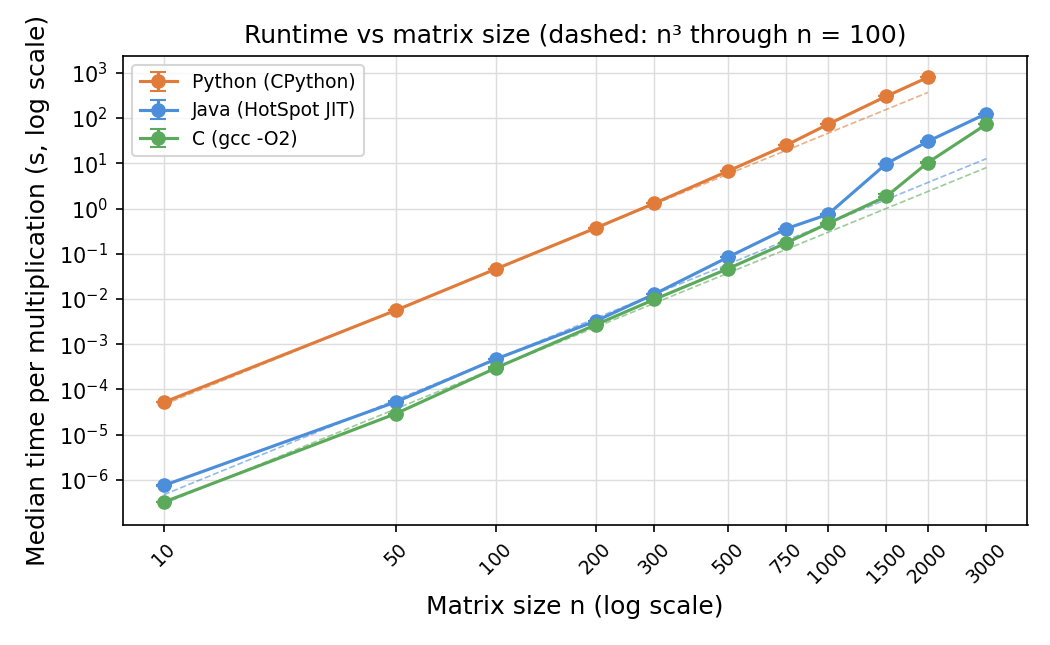
\includegraphics[width=0.8\textwidth]{../results/plot_time.png}
    \caption{Median time per multiplication vs matrix size $n$ (log-log scale). Dashed
    lines show the cubic model $t \propto n^3$ through each language's median at
    $n = 100$. Error bars show the IQR (mostly smaller than the markers).}
    \label{fig:time}
\end{figure}

\begin{figure}[htbp]
    \centering
    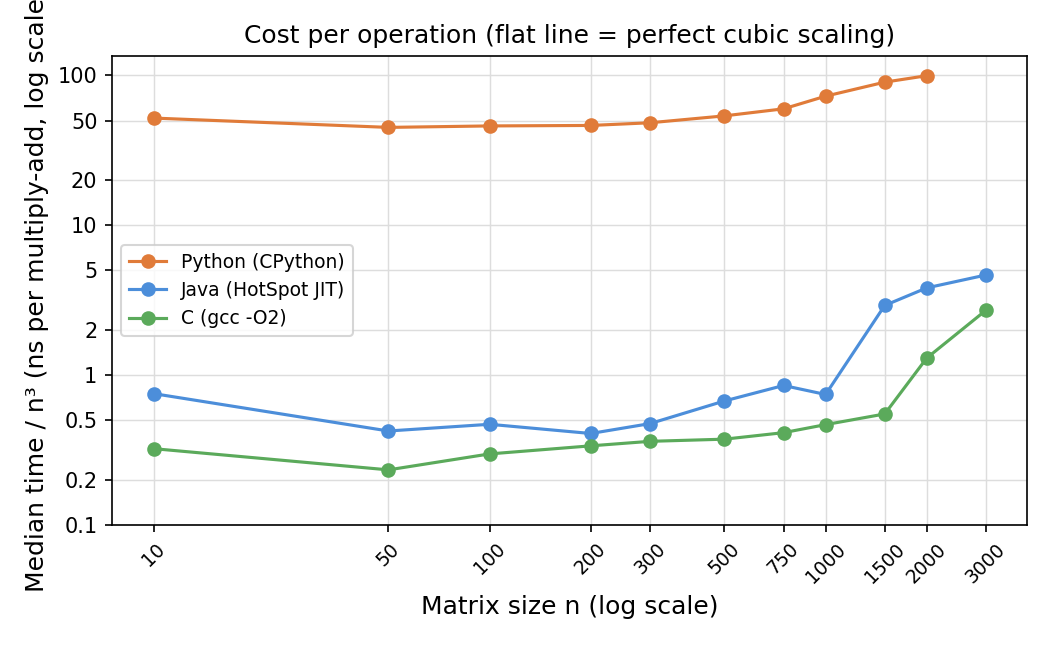
\includegraphics[width=0.8\textwidth]{../results/plot_cost_per_op.png}
    \caption{Median time divided by $n^3$ (nanoseconds per multiply-add). If the runtime
    were exactly proportional to $n^3$, each line would be horizontal.}
    \label{fig:costperop}
\end{figure}

\textit{Variability.} The IQR is at most 4.0\% of the median in every configuration except
C at $n = 1500$ (12.1\%), $n = 100$ (7.0\%) and $n = 10$ (4.5\%). At $n = 1500$ the C runs
agree within 1\% inside each process, but the three process medians are 1.81, 1.86 and
2.05~s (spread 12.8\%); in all other configurations with three processes the process
medians differ by at most 6.6\%. The Java slowdown at $n = 1500$ appears in all three
processes (medians 9.86, 9.56 and 9.92~s).

\textit{Growth.} A least-squares fit of $\log t$ against $\log n$ gives exponents of 3.18
(C), 3.30 (Java) and 3.19 (Python) for $100 \le n \le 1000$, and 4.69, 4.62 and 3.46 for
$n \ge 1000$. Because the second fit mixes segments with very different behaviour,
Table~\ref{tab:segments} gives the exponent between consecutive sizes. Doubling $n$ from
100 to 200 multiplies the time by 9.1 (C), 6.9 (Java) and 8.1 (Python); from 1000 to
2000, by 22.2, 41.2 and 11.0.

\begin{table}[htbp]
\centering
\small
\begin{tabular}{lrrrrrr}
\toprule
& \multicolumn{2}{c}{\textbf{C}} & \multicolumn{2}{c}{\textbf{Java}}
& \multicolumn{2}{c}{\textbf{Python}} \\
\textbf{Segment} & \textbf{exp.} & \textbf{ns at end} & \textbf{exp.} & \textbf{ns at end}
& \textbf{exp.} & \textbf{ns at end} \\
\midrule
\tableinput{../results/tables/segments.tex}
\bottomrule
\end{tabular}
\caption{Growth exponent between consecutive sizes, $\log(t_2/t_1)/\log(n_2/n_1)$, and
time per multiply-add at the end of the segment (ns).}
\label{tab:segments}
\end{table}

\textit{Warm-up and allocation.} The Java warm-up rule stopped after 2 to 8 runs, never at
the maximum; the first warm-up run was 2.4 times the median at $n = 200$ and within 3\% of
it from $n = 750$. In C and Python it was within 7\% and 2\% of the median. The
\texttt{tracemalloc} call took 9.8--13.2 times as long as the median timed run. The
allocation of the result matrix alone took 40\% of the Java kernel time at $n = 10$,
3.7\% at $n = 100$ and less than 1\% from $n = 300$; in Python, 1.7\% at $n = 10$ and
less than 0.05\% from $n = 50$.

\subsection{Memory}

Table~\ref{tab:memory} gives both kinds of memory metric, and Figures~\ref{fig:peak}
and~\ref{fig:memory} show them. For $n \ge 1000$, a least-squares fit of the peak
against $n^2$ gives 24.0 bytes per element in C, 32.7 in Java and 123.3 in Python. Below
that size the peak is dominated by a fixed part: about 3.6~MiB for C and 17~MiB for the
Python interpreter. The Java peak falls from 199~MiB at $n = 10$ to 48~MiB at $n = 200$
before growing again: at the batched sizes, each batch leaves thousands of result
matrices as garbage, and the G1 collector lets the heap grow before collecting them.

\begin{table}[htbp]
\centering
\small
\begin{tabular}{rrrrrrr}
\toprule
& \multicolumn{3}{c}{\textbf{Peak working set (MiB)}}
& \multicolumn{3}{c}{\textbf{Language-specific (KiB)}} \\
\textbf{n} & \textbf{C} & \textbf{Java} & \textbf{Python} & \textbf{C: computed}
& \textbf{Java: heap} & \textbf{Py: tracemalloc} \\
\midrule
\tableinput{../results/tables/memory.tex}
\bottomrule
\end{tabular}
\caption{Memory per configuration. Left: peak working set of the process, the same
metric in the three languages (median over processes, MiB $= 2^{20}$ bytes). Right: the
three different language-specific metrics of Section~3.5 (KiB $= 1024$ bytes), not
comparable with each other.}
\label{tab:memory}
\end{table}

\begin{figure}[htbp]
    \centering
    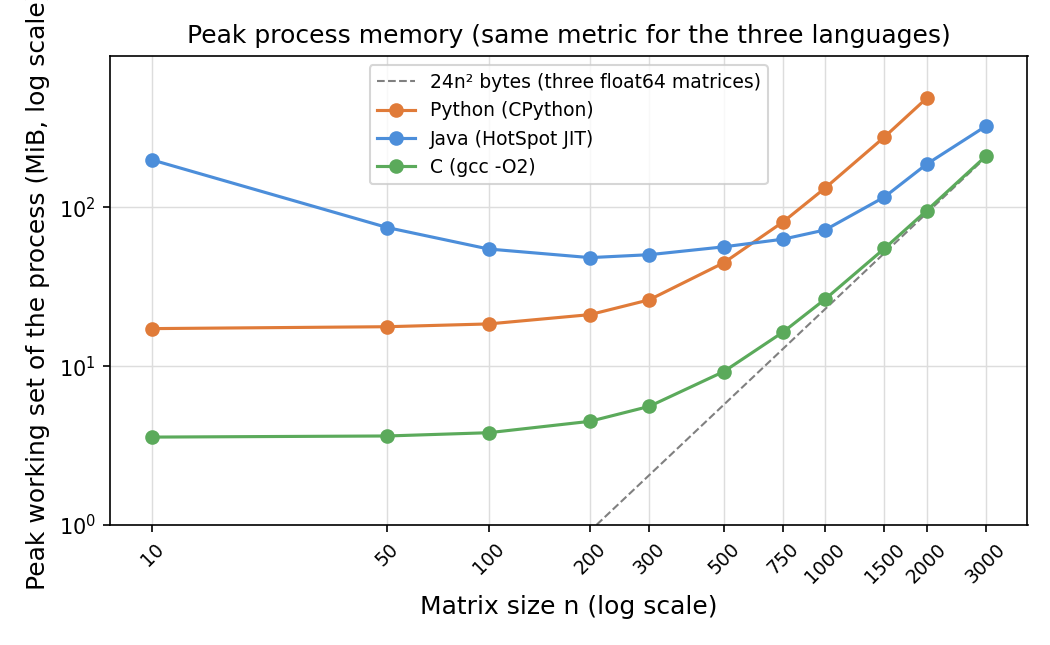
\includegraphics[width=0.8\textwidth]{../results/plot_peak_memory.png}
    \caption{Peak working set of the process vs matrix size $n$ (log-log scale), the
    same metric for the three languages. The dashed line is the storage of three
    float64 matrices, $24n^2$ bytes.}
    \label{fig:peak}
\end{figure}

\begin{figure}[htbp]
    \centering
    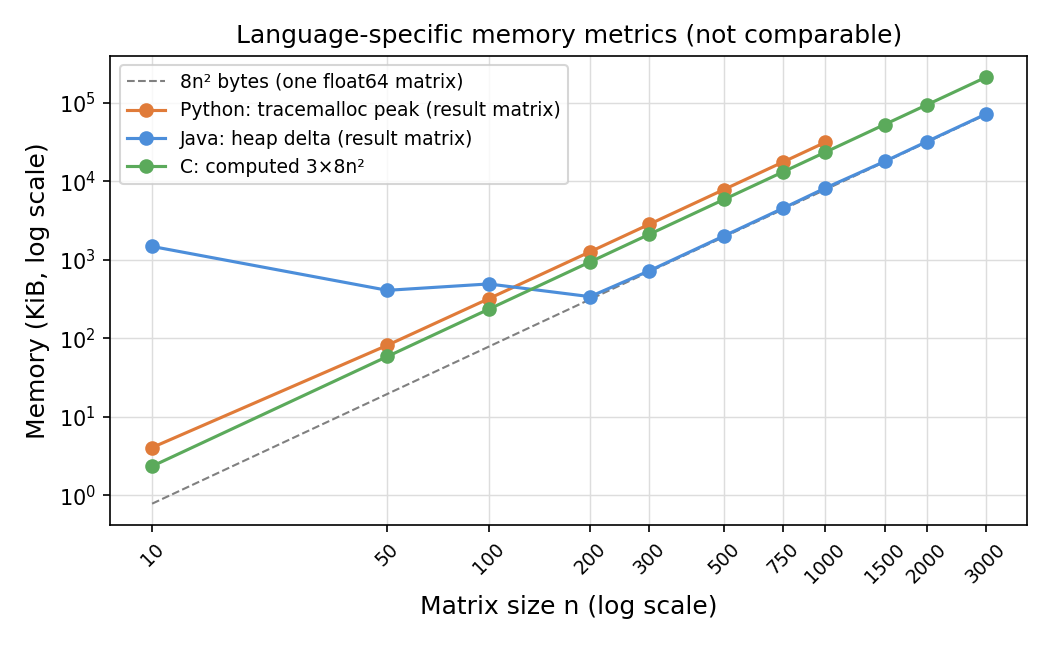
\includegraphics[width=0.8\textwidth]{../results/plot_memory.png}
    \caption{Language-specific memory metrics vs matrix size $n$ (log-log scale); the
    legend names the metric of each language. The dashed line is the storage of one
    float64 matrix, $8n^2$ bytes.}
    \label{fig:memory}
\end{figure}

\subsection{Largest feasible size}

Table~\ref{tab:limits} shows the largest size that finished within the budget and the
first size that exceeded it.

\begin{table}[htbp]
\centering
\small
\begin{tabular}{llll}
\toprule
\textbf{Language} & \textbf{Largest feasible $n$} & \textbf{Longest run} &
\textbf{First size over budget} \\
\midrule
C      & 3000 & 74~s ($n = 3000$)  & none \\
Java   & 3000 & 126~s ($n = 3000$) & none \\
Python & 2000 & 797~s ($n = 2000$) & 3000 (TIMEOUT at 900~s) \\
\bottomrule
\end{tabular}
\caption{Limits under the 15-minute-per-run budget (\texttt{results/run\_status.csv}).
The largest size attempted was $n = 3000$ in all three languages. The largest peak
working set was 485~MiB (Python, $n = 2000$), far below the 30~GB budget.}
\label{tab:limits}
\end{table}

\FloatBarrier
\section{Discussion}

\subsection{Evaluation of the hypotheses}

In answer to the research question: runtime grows as $n^3$ only up to a size that depends
on the implementation, memory grows with $n^2$ by an amount per element set by each
storage layout, and the language changes the runtime by a factor that depends on $n$.
Table~\ref{tab:verdicts} gives the verdict for each prediction.

\begin{table}[H]
\centering
\small
\begin{tabular}{p{2.2cm}p{8.0cm}>{\raggedright\arraybackslash}p{3.0cm}}
\toprule
\textbf{Prediction} & \textbf{Observed} & \textbf{Verdict} \\
\midrule
Cubic growth & Exponents 3.18--3.30 for $100 \le n \le 1000$; the cost per operation
jumps from $n = 1500$ in Java and from $n = 2000$ in C & Partly confirmed (only for
$100 \le n \le 1000$) \\
\addlinespace
Language ranking & C $<$ Java $<$ Python at every size. Java 1.2--2.1 times C for
$100 \le n \le 1000$, 5.3 at $n = 1500$. Python 134--193 times C up to $n = 1500$ &
Partly confirmed (order correct, gaps not) \\
\addlinespace
Memory per element & Slope of the peak against $n^2$: 24.0~B (C), 32.7~B (Java),
123.3~B (Python) & Confirmed for C and Python; Java above \\
\bottomrule
\end{tabular}
\caption{Verdict for each prediction of Table~\ref{tab:predictions}.}
\label{tab:verdicts}
\end{table}

\subsection{Growth with matrix size}

For $100 \le n \le 1000$ the exponents (3.18--3.30) and the doubling factors (6.9--9.1)
are close to the cubic model. Beyond, the number of operations still follows $n^3$, so
the faster growth means that each operation becomes more expensive. The segments of
Table~\ref{tab:segments} locate the change: in C the cost per operation rises slowly up
to $n = 1500$ (0.55~ns) and jumps between 1500 and 2000 (1.30~ns, exponent 5.98); in Java
the jump comes one step earlier, between 1000 and 1500 (0.74 to 2.92~ns, exponent 6.38).
The single fit over $n \ge 1000$ averages these segments and is not a growth law.

Two effects of the column walk over $B$ are consistent with the position of the jump in
C, and the data cannot tell them apart. \textit{L3 capacity:} each row of the result
reads the whole of $B$ again, and $B$ occupies $8n^2$ bytes, 18~MB at $n = 1500$, which
fits in the 30~MB L3, and 32~MB at $n = 2000$, which does not; from then on $B$ comes from
main memory for every row~\cite{hennessy2019}. \textit{Address translation:} one column
walk touches $n$ different pages (2000 at $n = 2000$), which may exceed what the TLB
holds~\cite{hennessy2019}. Separating them would need hardware counters or large pages,
so both remain hypotheses. The process-to-process spread of C at $n = 1500$, at the edge
of this transition, is consistent with each process receiving a different placement of
its pages in physical memory, which changes how the matrices map onto the cache; this was
not measured either, but it shows why repetitions in independent processes were needed.

At the smallest sizes fixed costs remain even with batches (in Java the allocation of
the result takes 40\% of the kernel time at $n = 10$), and the Java warm-up needed up to
8 runs, consistent with the JIT compiler replacing interpreted code over several
calls~\cite{oraclejvm}.

\subsection{Differences between languages}

\textit{Java vs C.} For $100 \le n \le 1000$ Java needs 1.2--2.1 times the C time: once
compiled, both execute native code. At $n = 1500$ the gap jumps to 5.3, reproducibly
across processes, because the Java cost per operation grows from 0.74 to 2.92~ns while
that of C grows from 0.47 to 0.55~ns. Both store 8-byte doubles; a plausible difference
is the access to $B$: in C its address is computed directly in one flat array, while in
Java each step first reads the reference to row $k$~\cite{jls21}, one more memory access
per operation, which may make Java reach the cache limit at a smaller $n$. The gap
narrows again at larger sizes (1.7 at $n = 3000$), when C is also limited by main memory.
The data cannot separate the layout from other JIT effects such as bounds checks, nor
explain the small drop of the Java cost at $n = 1000$.

\textit{Python vs C.} Python needs 134--193 times the C time up to $n = 1500$, above the
predicted 10--100. CPython spends about 45~ns per multiply-add for small matrices against
0.2--0.3~ns in C, because each operation is a sequence of bytecode instructions run by
the interpreter~\cite{pydis} and produces a new float object~\cite{pydatamodel}. This
cost grows only gradually with $n$ (45 to 100~ns), and the ratio drops to 77 at
$n = 2000$ only because C slows down.

\subsection{Memory}

Only the peak process memory is comparable between languages. Each additional element
raises it by 24.0~bytes in C, exactly the three float64 matrices predicted, and by
123.3~bytes in Python, above the predicted minimum of 96: under this metric an element
costs about five times as much in Python as in C. The remaining 27~bytes are not
explained by the measurements; the temporary list built while generating the inputs and
memory retained by the Python allocator are possible causes. In Java the slope, 32.7
bytes, exceeds the prediction by about one matrix of doubles, consistent with result
matrices that are garbage but not yet collected. The language-specific metrics agree with
the layouts but measure different things: 8.1--8.7 bytes per element for the Java heap
delta (a result of doubles) and 32.1--32.3 for the Python \texttt{tracemalloc} peak (a
result of references and float objects), while the C value is 24 by definition. The Java
heap values for $n \le 100$ are dominated by allocation buffers and are not meaningful.

\subsection{Limitations}

\begin{itemize}
    \item One Windows computer and one set of language versions; other cache sizes would
    move the jumps in the cost per operation. The power plan was the default
    \textit{Balanced}, not a fixed frequency.
    \item The most expensive configurations have only 5 runs in one process (C and Java at
    $n = 3000$, Python at $n = 1000$) or 3 (Python at $n \ge 1500$); C at $n = 1500$
    shows that single-process runs may underestimate the uncertainty.
    \item The cache, TLB and Java-layout explanations are inferred from timings only.
    \item The peak working set depends, in Java, on when the garbage collector runs; the
    Python language-specific metric stops at $n = 1000$.
    \item C and Java still ran far below the budget at $n = 3000$ (74~s and 126~s), so
    their actual largest feasible size was not determined.
\end{itemize}

\section{Conclusions}

For the three implementations and the conditions described in Section~3:
\begin{itemize}
    \item For $100 \le n \le 1000$ the runtime agrees with the $n^3$ model (exponents
    3.18--3.30). The cost per operation then jumps, from $n = 1500$ in Java and from
    $n = 2000$ in C, so it depends on the matrix size and not only on the number of
    operations.
    \item C is the fastest at every size. Java needs 1.2--2.1 times the C time for
    $100 \le n \le 1000$, 5.3 times at $n = 1500$ and 1.7 times at $n = 3000$. Python
    needs 134--193 times the C time up to $n = 1500$, more than predicted.
    \item For large $n$, the peak process memory grows by 24~bytes per matrix element in
    C, about 33 in Java and about 123 in Python.
    \item Under the 15-minute budget, C and Java completed every declared size up to
    $n = 3000$, and Python up to $n = 2000$.
\end{itemize}
These results compare specific implementations on one machine, not programming languages
in general. Two questions remain open: whether the jump in the cost per operation comes
from the L3 capacity, from address translation or from both, and how much of the Java--C
gap comes from the \texttt{double[][]} layout. Both are starting points for the
loop-reordering and blocking optimisations~\cite{hennessy2019} of Assignment~2.

\section*{Reproducibility materials}

The repository linked on the first page contains the source code, the build and run
commands (\texttt{README.md}) and, in \texttt{results}, the raw measurements of every
run, the status and peak memory of every process, the allocation timings, the
environment record and the correctness results. The study is reproduced on Windows with
\texttt{run\_experiment.py} (build and benchmarks), the validation script
\texttt{analysis/check\_correctness.py}, \texttt{analysis/plot\_results.py} (figures
and tables) and \texttt{analysis/report\_numbers.py} (every other number in the text).

\section*{Use of generative AI}

Claude Sonnet 4.6 and Claude Opus 5.5 (Anthropic), used through Claude Code, served as
support tools during this assignment: to help write and debug parts of the benchmark and
analysis scripts, and to improve the structure and wording of the report. All the
measurements come from running the code on the machine described above. The author
reviewed the code and the AI-generated text, checked the numbers against the raw data and
the references, and is responsible for the conclusions.

\clearpage
{\small
\begin{thebibliography}{8}

\bibitem{cormen2009}
T.~H. Cormen, C.~E. Leiserson, R.~L. Rivest, and C.~Stein, \textit{Introduction to
Algorithms}, 3rd~ed. Cambridge, MA, USA: MIT Press, 2009.

\bibitem{hennessy2019}
J.~L. Hennessy and D.~A. Patterson, \textit{Computer Architecture: A Quantitative
Approach}, 6th~ed. Cambridge, MA, USA: Morgan Kaufmann, 2019.

\bibitem{oraclejvm}
Oracle, ``Java HotSpot virtual machine performance enhancements,'' in \textit{Java
Virtual Machine Guide, Release~21}. [Online]. Available:
\url{https://docs.oracle.com/en/java/javase/21/vm/java-hotspot-virtual-machine-performance-enhancements.html}.

\bibitem{pydatamodel}
Python Software Foundation, ``Data model,'' in \textit{The Python Language Reference},
Python~3.11 documentation. [Online]. Available:
\url{https://docs.python.org/3.11/reference/datamodel.html}.

\bibitem{pydis}
Python Software Foundation, ``dis --- Disassembler for Python bytecode,'' in \textit{The
Python Standard Library}, Python~3.11 documentation. [Online]. Available:
\url{https://docs.python.org/3.11/library/dis.html}.

\bibitem{jls21}
J.~Gosling \textit{et al.}, ``Chapter~10: Arrays,'' in \textit{The Java Language
Specification, Java SE 21 Edition}. Oracle, 2023. [Online]. Available:
\url{https://docs.oracle.com/javase/specs/jls/se21/html/jls-10.html}.

\bibitem{gccopt}
Free Software Foundation, ``Options that control optimization,'' in \textit{Using the GNU
Compiler Collection (GCC)}. [Online]. Available:
\url{https://gcc.gnu.org/onlinedocs/gcc/Optimize-Options.html}.

\bibitem{goldberg1991}
D.~Goldberg, ``What every computer scientist should know about floating-point
arithmetic,'' \textit{ACM Comput. Surv.}, vol.~23, no.~1, pp.~5--48, Mar. 1991,
doi: 10.1145/103162.103163.

\end{thebibliography}
}

\end{document}
